%----------------------------------------------------------------------------------------
%   PACKAGES AND DOCUMENT CONFIGURATIONS
%----------------------------------------------------------------------------------------

\documentclass[12pt]{article}
\usepackage[english]{babel}
\usepackage[utf8]{inputenc}
\usepackage{float}

\usepackage{graphicx,epstopdf}   %for embedding images and for conveting eps to pdf
\usepackage{subfig}              %for sub images
\usepackage[margin=1in,includefoot]{geometry}	%changes the margins of report to 1 in
\usepackage{lscape}

\usepackage{rotating}   %used for rotating figures
\usepackage[automake,nonumberlist]{glossaries}    %To use glossary
\usepackage{varwidth}
\usepackage{multicol}   %for making columns
\usepackage{amsmath}
\usepackage{appendix}
\usepackage{lipsum}

\usepackage[framed, numbered]{matlab-prettifier}    %to import matlab code

%----------------------------------------------------------------------------------------
%   Acronym/Glossary
%----------------------------------------------------------------------------------------
\makeglossaries
\loadglsentries{glossary}

%----------------------------------------------------------------------------------------
%   Document Start
%----------------------------------------------------------------------------------------

\begin{document}

\begin{titlepage}

\newcommand{\HRule}{\rule{\linewidth}{0.5mm}} % Defines a new command for the horizontal lines, change thickness here

\center % Center everything on the page
 
%----------------------------------------------------------------------------------------
%   HEADING SECTIONS
%----------------------------------------------------------------------------------------

\textsc{\LARGE MSE 450 Real Time and Embedded Control Systems}\\[1.5cm] % Org Name
\textsc{\Large }\\[0.5cm] % course name
\textsc{\large }\\[0.5cm] % course title

%----------------------------------------------------------------------------------------
%   TITLE SECTION
%----------------------------------------------------------------------------------------

\HRule \\[0.4cm]
{ \huge \bfseries Design Report}\\[0.4cm] % Title of report
\HRule \\[1.5cm]
 
%----------------------------------------------------------------------------------------
%   AUTHOR SECTION
%----------------------------------------------------------------------------------------

\begin{minipage}{0.4\textwidth}
    \begin{flushleft} \large
        \emph{Authors:}\\
        Parshant \textsc{Bombhi}\\
        Jigar \textsc{Jhankharia}\\
        Mitchell \textsc{Humphrey}
    \end{flushleft}
\end{minipage}
\hfill
\begin{minipage}{0.4\textwidth}
    \begin{flushright} \large
        \emph{Student ID:} \\
        301255126\\
        301215232\\
        301281152
    \end{flushright}
\end{minipage}
\vspace{10mm}
%----------------------------------------------------------------------------------------
%   DATE SECTION
%----------------------------------------------------------------------------------------

{\large \today}\\[2cm] % Date, change the \today to a set date if you want to be precise

%----------------------------------------------------------------------------------------
%   LOGO SECTION
%----------------------------------------------------------------------------------------


\includegraphics[scale=2.0]{MSE-Logo.jpg}\\[1cm] %logo
%----------------------------------------------------------------------------------------

\vfill % Fill the rest of the page with whitespace

\end{titlepage}

%----------------------------------------------------------------------------------------
%   Table of Contents/Table of Figures
%----------------------------------------------------------------------------------------
\pagenumbering{roman} %sets numbering of page to roman
\tableofcontents	%makes table of contents
\addcontentsline{toc}{section}{\numberline{}Table Of Contents}	%adds TOC to TOC

%\listoffigures
%\addcontentsline{toc}{section}{\numberline{}List of Figures}	%adds list of figures to table of contents

 %\listoftables
 %\addcontentsline{toc}{section}{\numberline{}List of Tables}

%\lstlistoflistings
%\addcontentsline{toc}{section}{\numberline{}Listings}

% \printglossary
% \addcontentsline{toc}{section}{\numberline{}Glossary}	%adds glossary to table of contents
\pagebreak
%----------------------------------------------------------------------------------------
%   Main Body
%----------------------------------------------------------------------------------------
\setcounter{page}{1}	%resets the page numbering
\pagenumbering{arabic}	%sets numbering of page to arabic
\setlength{\parskip}{1em}

\section{Abstract}
This report details the design specifications of a real-time controller for a 1-DOF pick and place robotic arm. We state the various components used and their purpose for this project. The hardware components include a DC motor, magnet, potentiometer, quadrature encoder, and a TM4C microcontroller. 
 
Our objective is to program the microcontroller to control the robotic arm. This will be done by sending voltage signals to the DC motor that will allow the arm to rotate. The use of the potentiometer is to sense the position of the arm and this can be set by the user as programmed. To pick and place any object a magnet is used as a grip.
 
The purpose of this project is to apply the material learnt in this course to a hands-on project and achieve real time results by the extensive use of interrupts. We will use a PID controller for this project and apply the theories learnt in class to achieve our objective. 

\section{Introduction}
As we develop a real-time controller for a 1-DOF pick and place robotic arm, we design this based on real time to see the difference between real-hard time and soft time. This is because in real world applications and dynamic system developments, timing is vital and otherwise turns to be catastrophic. This pick and place robot arm will be controlled using a PID controller that will be responsible for the exact positioning and balancing of the objects that are getting picked and place in another position in real time. 
 
In real-world applications, controlling a dynamic system is extremely important with the advances in technology. Real-time control is vital for systems that have a strict timing requirement. For our project, we will develop a real-time controller for a 1-DOF pick and place robotic arm. A 1-DOF pick and place robotic arm is a robotic system that can be positioned to pick and place an object for performing a useful task. The controller is responsible for balancing and positioning the robotic arm in real-time. The setup we will be using consists of a DC motor attached to robotic arm, magnet, potentiometer, quadrature encoder, and a TM4C microcontroller.

\section{Design Goals and Objectives}
\subsection{Goals}
The goal of this project is:
\begin{itemize}
    \item Design a microcontroller to control a robotic arm. This controller would be a PID controller.
    \item Using Calibration techniques to calibrate the arm.
    \item Reading data user to the potentiometer to assign a position to the arm
    \item Apply voltage to the motor by sending PWM signals to the motor
    \item Activate and deactivate the magnet i.e. the grip to hold an object
\end{itemize}
\subsection{Objectives}
\begin{itemize}
    \item Understanding and visually being able to see real-time embedded system applications
    \item Applying the theories and techniques learnt in class
\end{itemize}
\section{Requirements}
This project has the following requirements to maximize the use of the robotic arm:
\begin{itemize}
    \item Pick and place magnetic objects from one position to another
    \item Use of a PID controller
    \item Calibrate the arm
    \item Use of the potentiometer to read the exact position of the arm
    \item Pulse Width Modulation to control the motor
    \item Use the potentiometer data periodically to update the microcontroller
\end{itemize}
\section{Method}
Practically the microcontroller will be used to control the arm once the code is added to the microcontroller. Therefore, to meet the requirements of a real-time systems we will extensively be using interrupts in our code. We will have 4 stages/system connections for this system to function as follows:
\begin{itemize}
    \item Stage 1 – Will be the user input
    \item Stage 2 – Microcontroller – TM4C123G
    \item Stage 3 – H-Bridge connection
    \item Stage 4 – Robotic Arm
\end{itemize}
To elaborate these stages, the user input is an angle input by the user that the robotic arm will correspond to i.e. follow the angle input once the information reaches the arm. The second stage is that the microcontroller will process the user input and send the data to the arm through stage 3 that is a H-bridge circuit. The H-bridge circuit is used to help determine the direction the arm should move in i.e. clockwise or anticlockwise direction.

Below is a flow chart determined to outline the process of the arm’s pick and place function.
\begin{figure}[H]
    \centering
    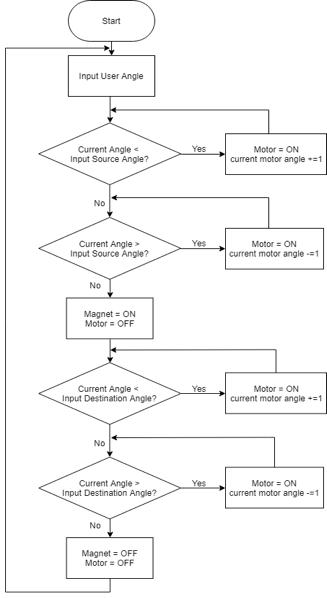
\includegraphics[width=0.5\textwidth]{450_design_report.png}
\end{figure}
\section{Platform and Tools}
For this project we will be making use of both a variety of hardware and software to build, develop, and control a 1-DOF robotic arm.

The hardware that we will make use of consists of a TM4C123 microcontroller (and it’s integrated functions), a DC motor, magnet, potentiometer, and quadrature encoder. The microcontroller, as you would expect, is to be used as the brain of the robot which we will also use for its pulse-width modulation (PWM) and analog-to-digital (ADC) processing. The microcontroller will use its the out PWM signal to control the DC motor’s position and velocity, and subsequently the entire motion of the arm. The potentiometer will be used in conjunction with the microcontrollers ADC processing to give the operator positioning control of the robot. The magnet will simply act as a pseudo-gripper for the arm. Lastly, the quadrature encoder will be providing feedback for the DC motor to allow for precise monitoring and adjustment of the robotic arm’s position.

As for the software, we will be using Code Composer Studio to program the microcontroller along with a PID controller to monitor and manage the feedback from the system. Code Composer will simply be the compiler for the program that we will develop to control the arm. The PID controller will be a software tool that we will use to manage the systems feedback and allow for a greater degree of precision.

\section{Implementation Plan and Timeline}
\begin{itemize}
    \item Begin assembly of the robotic arm on March 14th
    \item Complete the assembly of the robot by March 17th
    \item Complete basic wiring and debugging by March 20th
    \item Complete programming by March 30th
    \item Conduct any Debugging on April 1st
    \item Perform the project demonstration on either April 2nd or 4th
    \item Complete project report by April 6th
\end{itemize}
\section{Conclusion}
In summation, for this project we intend to assemble, develop, and program a 1-DOF robotic arm using a TM4C123 microcontroller with a PID controller to run it. The first objective of this project is to make a robot that has precise position feedback and is controllable via a potentiometer. The second objective is to apply the knowledge that we developed in class, as well as, to gain a deeper understanding of it through application. We expect to be able to follow the timeline laid forth earlier in this report without much difficulty as we have factored in extra time in each stage for any challenges that may crop up as we work. We look forward to the outcome of this project and what we will learn along the way.
\end{document}
              
            